% Chapter Template

\chapter{Classification Stability} % Main chapter title

\label{Chapter:Stability} % Change X to a consecutive number; for referencing this chapter elsewhere, use \ref{ChapterX}

%----------------------------------------------------------------------------------------
%	SECTION 1
%----------------------------------------------------------------------------------------

In this chapter we present a stability study done using our best performance algorithm. Deep learning models act many times as black box prediction machines that are trained using, many times, a large but finite training set. The purpose of the analysis presented in this chapter is study how the prediction capabilities of the model are affected by changes in the properties of input images. Learning about this behavior gives a better understanding of the robustness and limitations of the designed model.

\section{Introduction}

Deep learning models are trained using an end-to-end automatic process that allows to learn the best internal representation (ie. the features and the optimal classifier) minimizing a predefined loss function. As a result, an optimal parameterized model is obtained. Such models typically have hundreds of thousands or millions of parameters, being difficult to interpret. The model validity is tested using a test data set hopefully coming from the same data distribution that the training set. Using a big enough test set of never seen before data, it is possible to corroborate the statistical validity of the results reported by the model. Such type of test gives us a overall understanding about the statistical performance, however it does not give us any information about the model behavior under variation of typical input image parameters like rotation, lightness, hue, saturation, zoom, etc. 

The purpose of this chapter is the study of results variability under typical changes in the input image parameters. This study allows a better understanding of the nature of trained models in order to increase its robustness and to know the intrinsic limitations of the trained models.

%\section{Background}

%Deep learning models in general are very vulnerable to adversarial examples \citep{kurakin2016adversarial}. An adversarial example is a conventional input that introduces slight modifications on some of its pixel values that produce a complete mis-classification on model prediction, being the modification imperceptible to the human eye. This is a well known limitation of deep learning models that make them prone to attacks. 

%In \citep{goodfellow2015adversarial} a demonstration of fast adversarial example generation is applied to GoogLeNet on ImageNet.  By adding an imperceptibly small vector whose elements are equal to the sign of the elements of the gradient of the cost function with respect to the input, is possible to change GoogLeNet’s classification of the image.  


\section{Methods}

First of all, the method used for testing model robustness consists on defining set of parameters that are considered important to test. For all the set of parameters an interval of variation is defined. For a set of images, representative of the population of study, new images are generated with the new parameters defined. Classification scores are calculated for every new image generated and a graphical representation of classification scores versus parameter values are also generated. With such plots it is possible the determine the stability of model results under typical variations of the input properties.

The image parameters that are studied in this chapter are: rotation, lightness, hue and saturation.

\paragraph{Rotation:} The model of study have been trained using data augmentation techniques that included random rotation. Therefore, the model should be robust to changes in image input rotation. Testing against such property will help us decide if multiple evaluations using different input rotated versions are required and also if results are seriously affected to changes of this variable or not. For each image, 360 evaluations have been done using different rotated versions of the same image, each one separated by 1 degree of rotation.

\paragraph{Hue, Lightness and Saturation:} The model uses as input a 3 channels red, green, blue (RGB) representation of the retina image. From a conceptual perspective, color space is sometimes better to be considered using another type of representation, ie. hue, lightness and saturation (HLS) color space (see figure \ref{sta:fig:hsl}). HLS aligns better with the way human vision perceives color-making attributes. Lightness representing the brightness relative to the brightness of a similarly illuminated white; hue referring to the attribute of a visual sensation according to which an area appears to be similar to one of the perceived colors: red, yellow, green, and blue, or to a combination of two of them; and saturation showing the colorfulness of a stimulus relative to its own brightness \citep{fairchild2013color}. Changes in each one of the variables HLS are done maintaining constant the others. For each variable 600 evaluations of the same image are done. Lightness and saturation varying linearly from 25\% to 175\% of the original image, and hue varying from -180 to +180 degrees of the original hue angle value. 

\begin{figure}[ht!]
	\centering
	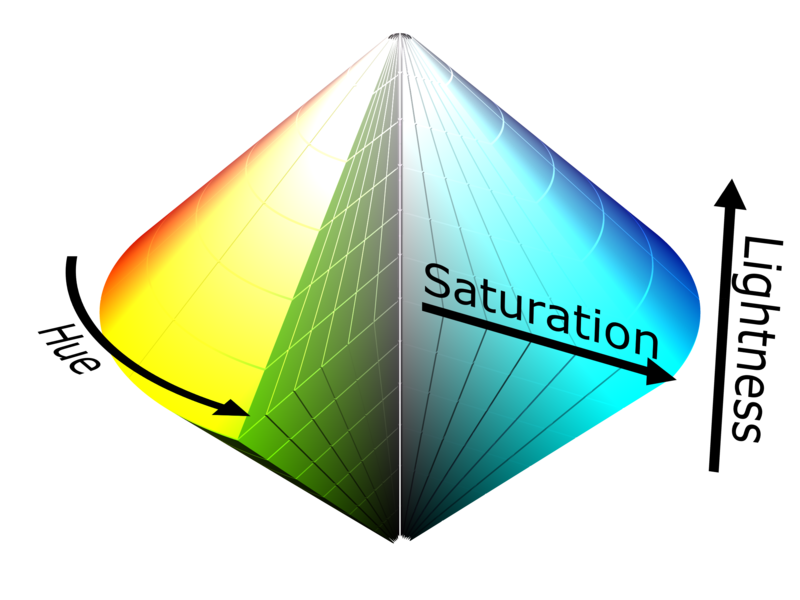
\includegraphics[width=0.5\textwidth]{Figures/chapter_stability/HSL_color_solid_dblcone.png}
	\caption[Hue-Lightness-Saturation color space cone]{Hue-Lightness-Saturation color space cone (source: commons.wikimedia.org)}
	\label{sta:fig:hsl}
\end{figure}

%-----------------------------------
%	SUBSECTION 2
%-----------------------------------

\section{Results}

The model used for the stability study is the one trained in chapter \ref{Chapter:Ordinal_Regression}. In the following subsections, stability results of the studied variables are reported. A random selection of images from the public Messidor Dataset \citep{decenciere_feedback_2014} have been chosen. Fig. \ref{sta:fig:imgs0} show the class 0 images selected for this study, fig. \ref{sta:fig:imgs1} the class 1, fig. \ref{sta:fig:imgs2} the class 2 and finally, fig. \ref{sta:fig:imgs3} the class 3 images. 

\begin{figure}[ht!]
	\centering
	%\scalebox{0.9}{
	\begin{subfigure}[b]{0.4\textwidth}
		\centering
		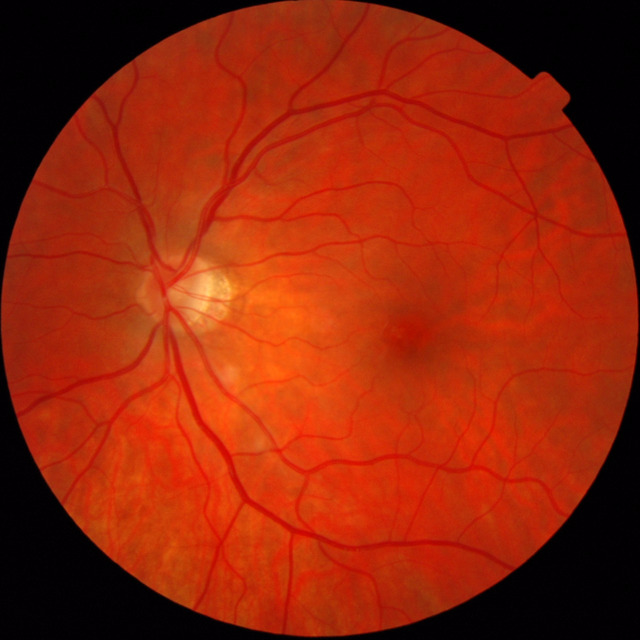
\includegraphics[width=\textwidth]{Figures/chapter_stability/20051020_62510_0100_PP/20051020_62510_0100_PP.jpeg}
		\caption{Messidor 20051020 62510 0100 PP Tag: 0}
	\end{subfigure} ~
	\begin{subfigure}[b]{0.4\textwidth}
		\centering
		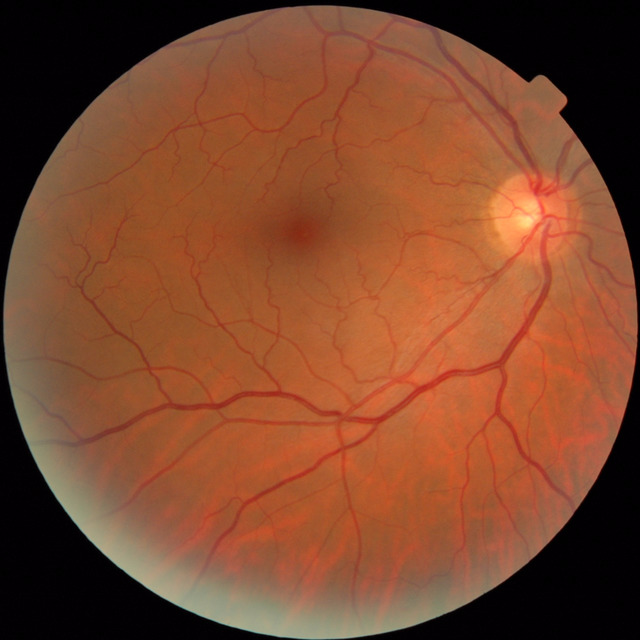
\includegraphics[width=\textwidth]{Figures/chapter_stability/20060523_45524_0100_PP/20060523_45524_0100_PP.jpeg}
		\caption{Messidor 20060523 45524 0100 PP Tag: 0}		
	\end{subfigure}	
	\begin{subfigure}[b]{0.4\textwidth}
		\centering
		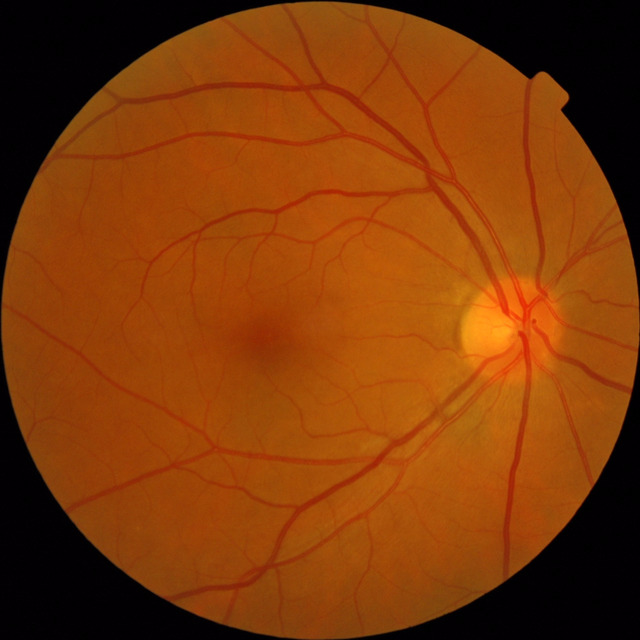
\includegraphics[width=\textwidth]{Figures/chapter_stability/20060523_48709_0100_PP/20060523_48709_0100_PP.jpeg}
		\caption{Messidor 20060523 48709 0100 PP Tag: 0}		
	\end{subfigure} ~
	\begin{subfigure}[b]{0.4\textwidth}
		\centering
		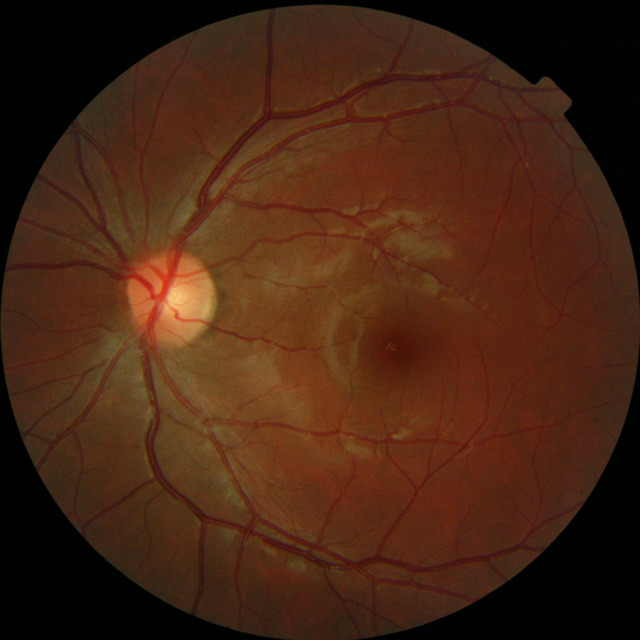
\includegraphics[width=\textwidth]{Figures/chapter_stability/20051130_59029_0400_PP/20051130_59029_0400_PP.jpeg}
		\caption{Messidor 20051130 59029 0400 PP Tag: 0}		
	\end{subfigure}
	%}
	\hfill 
	\caption{Images used for testing model robustness (Tag: 0)}  
	\label{sta:fig:imgs0} 
\end{figure}


\begin{figure}[ht!]
	\centering
	%\scalebox{0.9}{
	\begin{subfigure}[b]{0.4\textwidth}
		\centering
		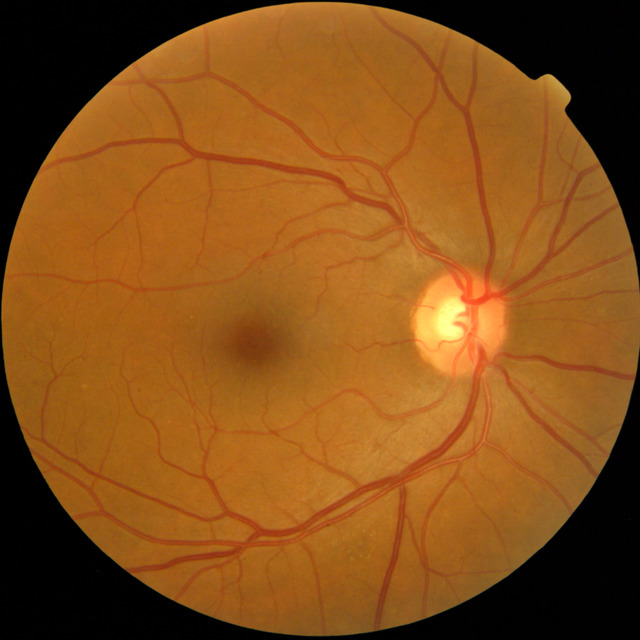
\includegraphics[width=\textwidth]{Figures/chapter_stability/20060412_61593_0200_PP/20060412_61593_0200_PP.jpeg}
		\caption{Messidor 20060412 61593 0200 PP Tag: 1}
	\end{subfigure} ~
	\begin{subfigure}[b]{0.4\textwidth}
		\centering
		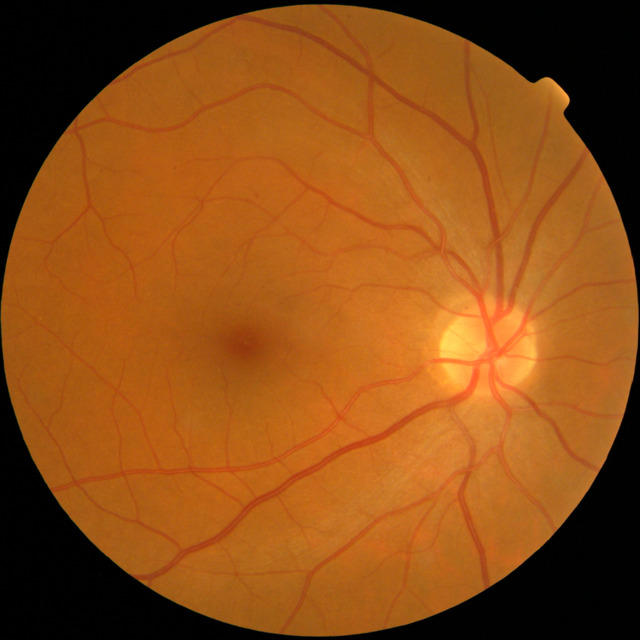
\includegraphics[width=\textwidth]{Figures/chapter_stability/20060411_62228_0200_PP/20060411_62228_0200_PP.jpeg}
		\caption{Messidor 20060411 62228 0200 PP Tag: 1}		
	\end{subfigure}	
	\begin{subfigure}[b]{0.4\textwidth}
		\centering
		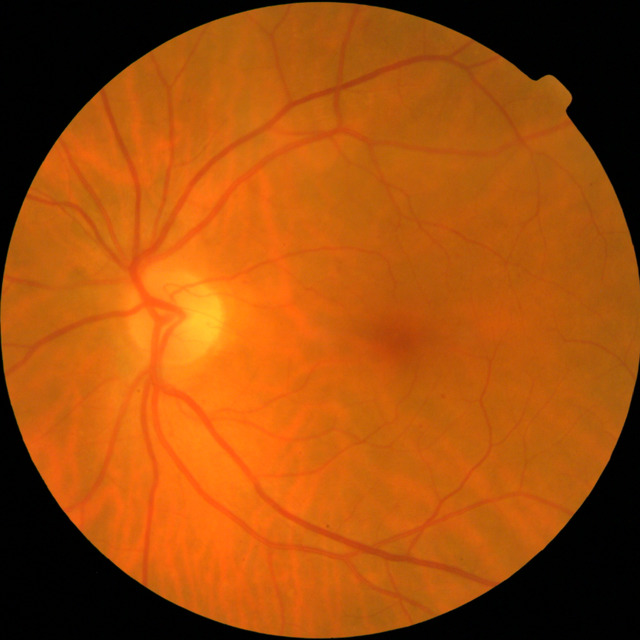
\includegraphics[width=\textwidth]{Figures/chapter_stability/20060412_59658_0200_PP/20060412_59658_0200_PP.jpeg}
		\caption{Messidor 20060412 59658 0200 PP Tag: 1}		
	\end{subfigure} ~
	\begin{subfigure}[b]{0.4\textwidth}
		\centering
		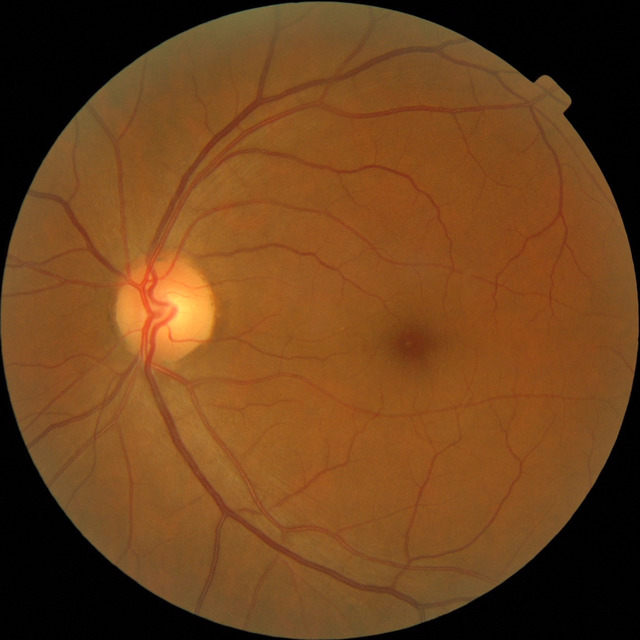
\includegraphics[width=\textwidth]{Figures/chapter_stability/20051020_44782_0100_PP/20051020_44782_0100_PP.jpeg}
		\caption{Messidor 20051020 44782 0100 PP Tag: 1}		
	\end{subfigure}
	%}
	\hfill 
	\caption{Images used for testing model robustness (Tag: 1)}  
	\label{sta:fig:imgs1} 
\end{figure}

\begin{figure}[ht!]
	\centering
	%\scalebox{0.9}{
	\begin{subfigure}[b]{0.4\textwidth}
		\centering
		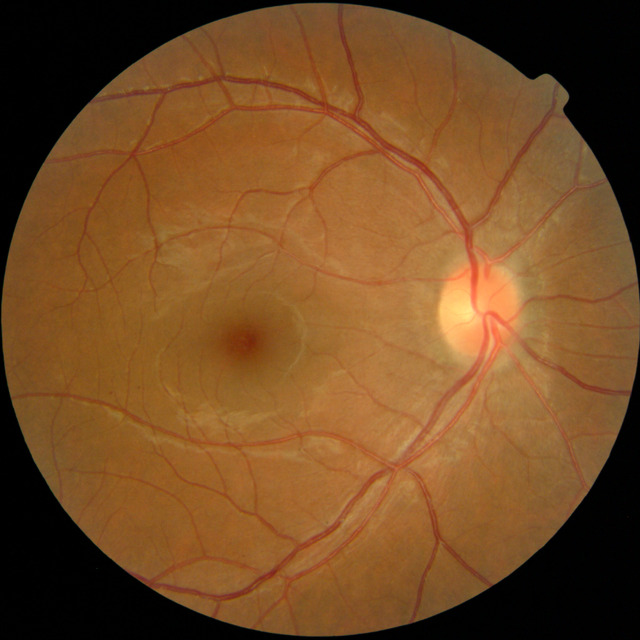
\includegraphics[width=\textwidth]{Figures/chapter_stability/20060410_40481_0200_PP/20060410_40481_0200_PP.jpeg}
		\caption{Messidor 20060410 40481 0200 PP Tag: 2}		
	\end{subfigure} ~
	\begin{subfigure}[b]{0.4\textwidth}
		\centering
		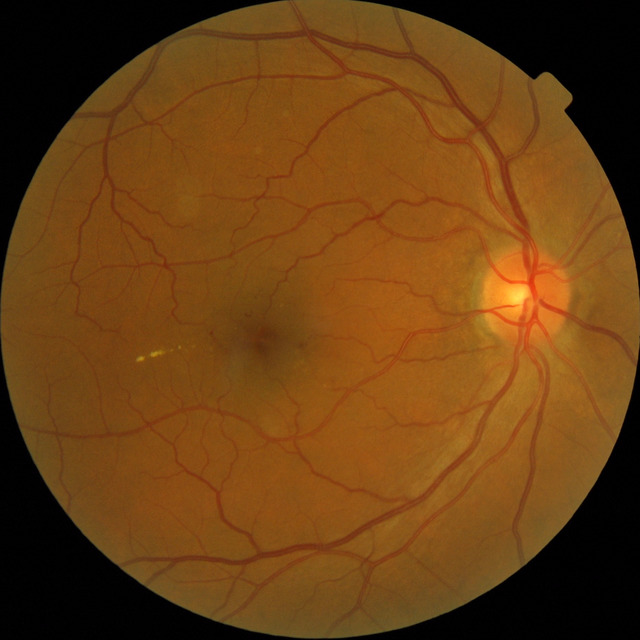
\includegraphics[width=\textwidth]{Figures/chapter_stability/20060523_50392_0100_PP/20060523_50392_0100_PP.jpeg}
		\caption{Messidor 20060523 50392 0100 PP Tag: 2}		
	\end{subfigure}
	
	\begin{subfigure}[b]{0.4\textwidth}
		\centering
		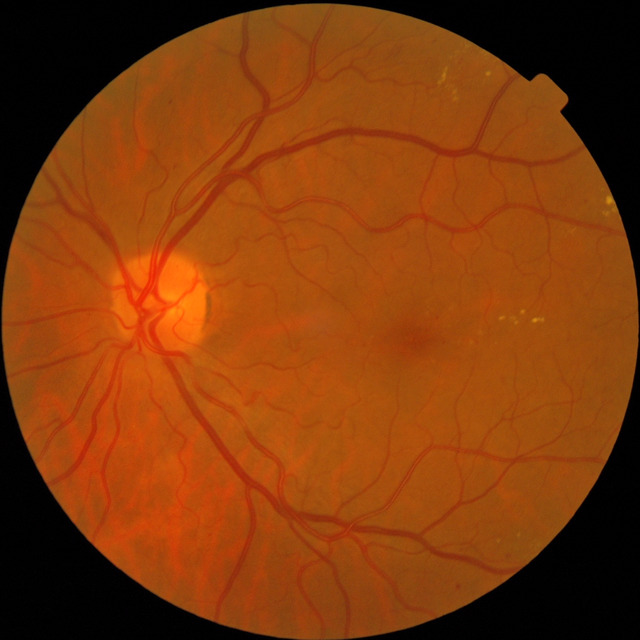
\includegraphics[width=\textwidth]{Figures/chapter_stability/20051214_57404_0100_PP/20051214_57404_0100_PP.jpeg}
		\caption{Messidor 20051214 57404 0100 PP Tag: 2}		
	\end{subfigure}	~
	\begin{subfigure}[b]{0.4\textwidth}
		\centering
		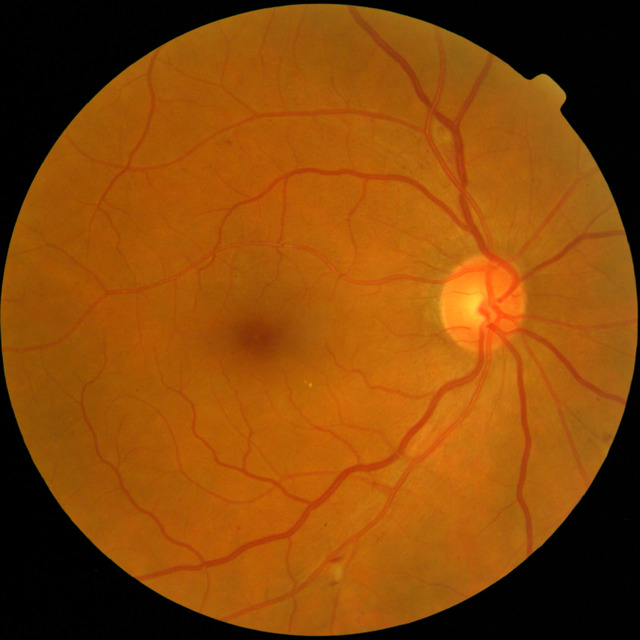
\includegraphics[width=\textwidth]{Figures/chapter_stability/20051216_44939_0200_PP/20051216_44939_0200_PP.jpeg}
		\caption{Messidor 20051216 44939 0200 PP Tag: 2}		
	\end{subfigure}
	%}
	\hfill 
	\caption{Images used for testing model robustness (Tag: 2)}  
	\label{sta:fig:imgs2} 
\end{figure}

\begin{figure}[ht!]
	\centering
	%\scalebox{0.9}{
	\begin{subfigure}[b]{0.4\textwidth}
		\centering
		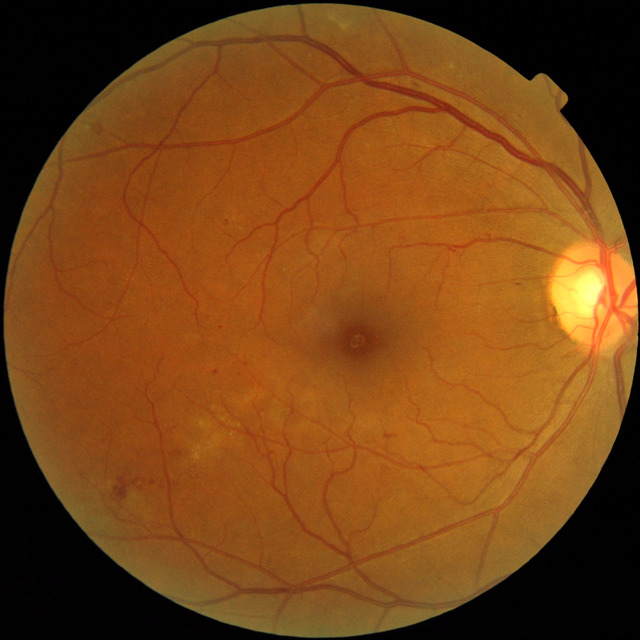
\includegraphics[width=\textwidth]{Figures/chapter_stability/20051019_38557_0100_PP/20051019_38557_0100_PP.jpeg}
		\caption{Messidor 20051019 38557 0100 PP Tag: 3}				
	\end{subfigure}	 ~
	\begin{subfigure}[b]{0.4\textwidth}
		\centering
		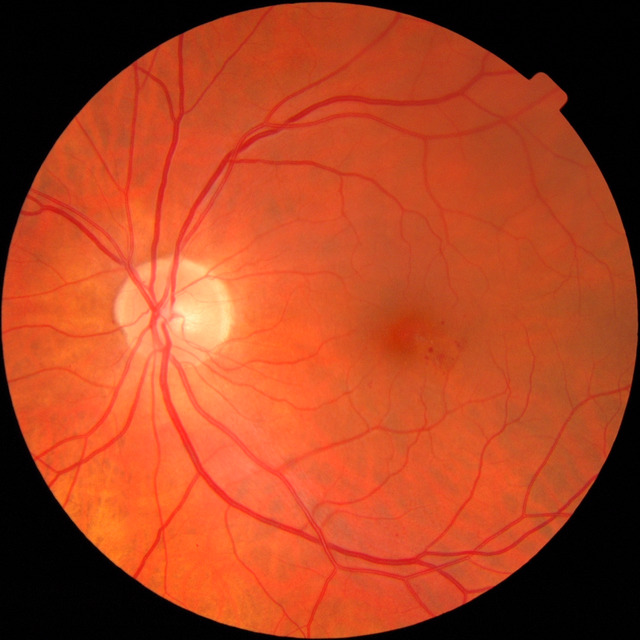
\includegraphics[width=\textwidth]{Figures/chapter_stability/20051020_43906_0100_PP/20051020_43906_0100_PP.jpeg}
		\caption{Messidor 20051020 43906 0100 PP Tag: 3}				
	\end{subfigure}	
	\begin{subfigure}[b]{0.4\textwidth}
		\centering
		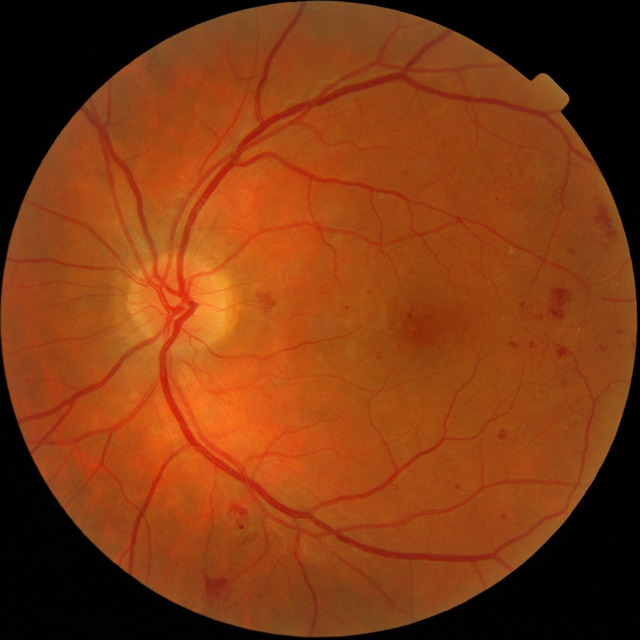
\includegraphics[width=\textwidth]{Figures/chapter_stability/20051021_52127_0100_PP/20051021_52127_0100_PP.jpeg}
		\caption{Messidor 20051021 52127 0100 PP Tag: 3}				
	\end{subfigure}	~
	\begin{subfigure}[b]{0.4\textwidth}
		\centering
		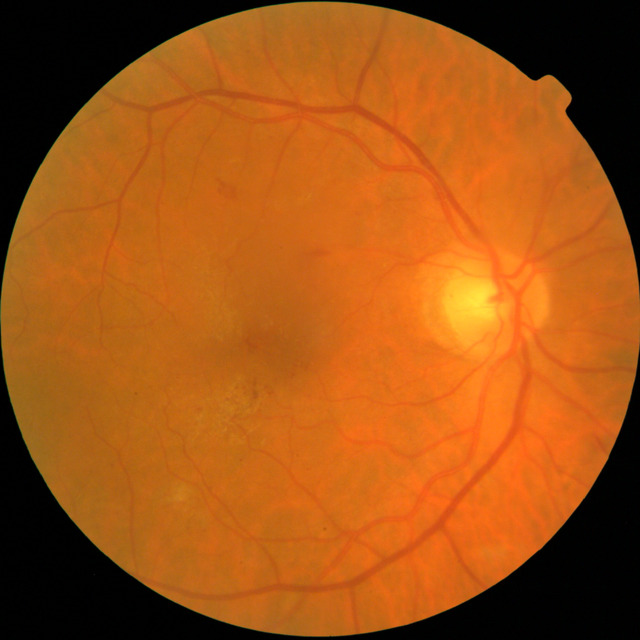
\includegraphics[width=\textwidth]{Figures/chapter_stability/20060412_59717_0200_PP/20060412_59717_0200_PP.jpeg}
		\caption{Messidor 20060412 59717 0200 PP Tag: 3}		
	\end{subfigure}
	%}
	\hfill 
	\caption{Images used for testing model robustness (Tag: 3)}  
	\label{sta:fig:imgs3} 
\end{figure}

\subsection{Rotation}

In the four class 0 analyzed samples (fig. \ref{sta:fig:rot0}), no change is observed in the value of predicted class when rotation is applied to the input image.  All four images are correctly classified as class 0 for all orientations. 

For class 1 (fig. \ref{sta:fig:rot1}), no change is observed in 3 of the 4 analyzed images, predicting the correct class in all of them for all orientations. In the fourth image a change in the score of predicted class is observed, changing between 0 and 1 class. The network arrive to different conclusions depending on orientation. In any case, the discrepancy is only of one class (between 0 and 1). The model predicts class 0 in 193 of the 360 rotations and class 1 in 167.

For class 2 (fig. \ref{sta:fig:rot2}), there is a discrepancy of one class distance between the tag and the predicted value in the first two images. The model predicts class 1 in the first image for all orientations, and for the second image predicts class 1 in 356 of the orientations and class 0 in 4 orientations. For the third and fourth images class 2 is correctly predicted for all the 360 rotated versions.

For class 3 (fig. \ref{sta:fig:rot3}), class 3 is correctly predicted in 3 of the 4 images, having a discrepancy of one class in the second image, predicted globally as class 2. Concretely, for the first image class 3 is predicted in 307 of the orientations and class 2 in 53. For the second, class 2 is predicted in 348 of the orientations and class 1 in 12.For the third, class 3 is predicted in all orientations. Finally in the fourth image, class 3 is predicted in 236 of the orientations and class 2 in 124.

\begin{figure}[ht!]
	\centering
	%\scalebox{0.9}{
	\begin{subfigure}[b]{ 0.85\textwidth}
		\centering
		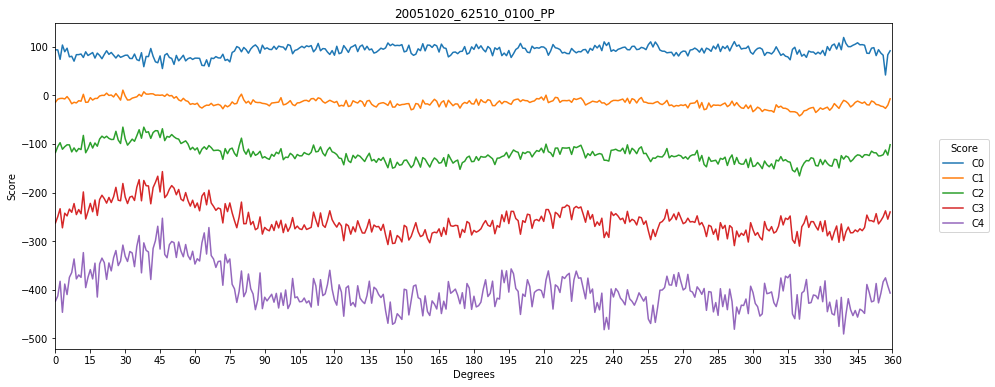
\includegraphics[width=\textwidth]{Figures/chapter_stability/20051020_62510_0100_PP/r/scores.png}
		\caption{Messidor 20051020 62510 0100 PP Tag: 0}
	\end{subfigure} 
	\begin{subfigure}[b]{ 0.85\textwidth}
		\centering
		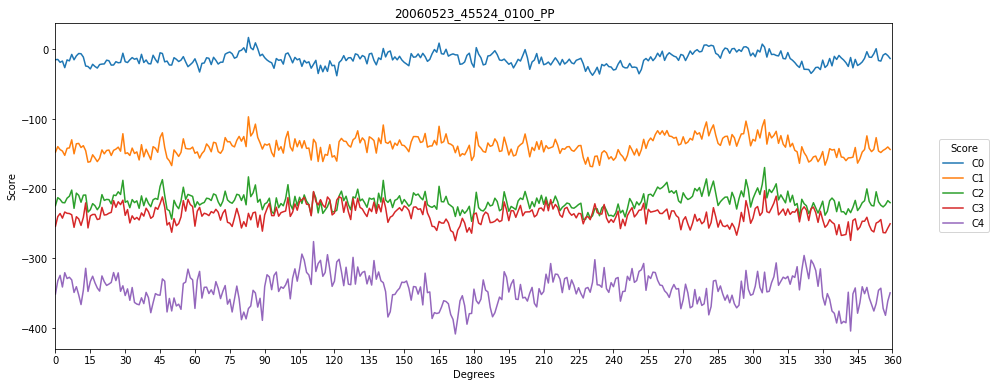
\includegraphics[width=\textwidth]{Figures/chapter_stability/20060523_45524_0100_PP/r/scores.png}
		\caption{Messidor 20060523 45524 0100 PP Tag: 0}		
	\end{subfigure}	
	\begin{subfigure}[b]{ 0.85\textwidth}
		\centering
		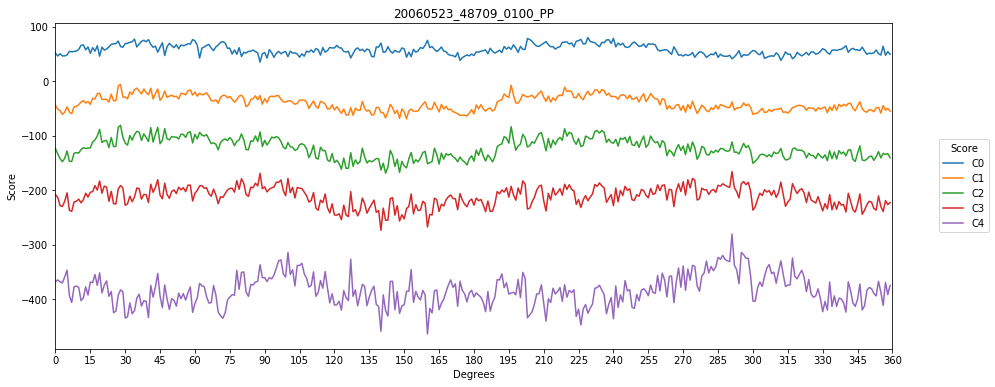
\includegraphics[width=\textwidth]{Figures/chapter_stability/20060523_48709_0100_PP/r/scores.png}
		\caption{Messidor 20060523 48709 0100 PP Tag: 0}		
	\end{subfigure} 
	\begin{subfigure}[b]{ 0.85\textwidth}
		\centering
		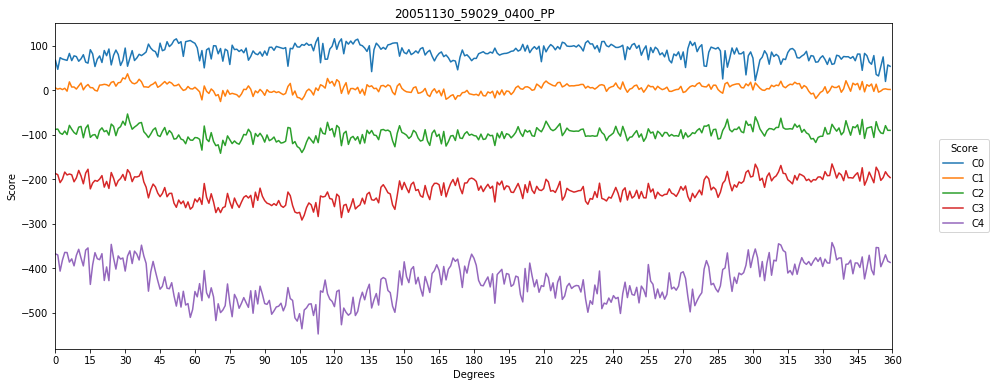
\includegraphics[width=\textwidth]{Figures/chapter_stability/20051130_59029_0400_PP/r/scores.png}
		\caption{Messidor 20051130 59029 0400 PP Tag: 0}		
	\end{subfigure}
	\hfill 
	%}
	\caption[Score vs Rotation (Tag: 0)]{Class Score vs Input Rotation (Tag: 0)}  
	\label{sta:fig:rot0} 
\end{figure}

\begin{figure}[ht!]
	\centering
	%\scalebox{0.9}{
	\begin{subfigure}[b]{ 0.85\textwidth}
		\centering
		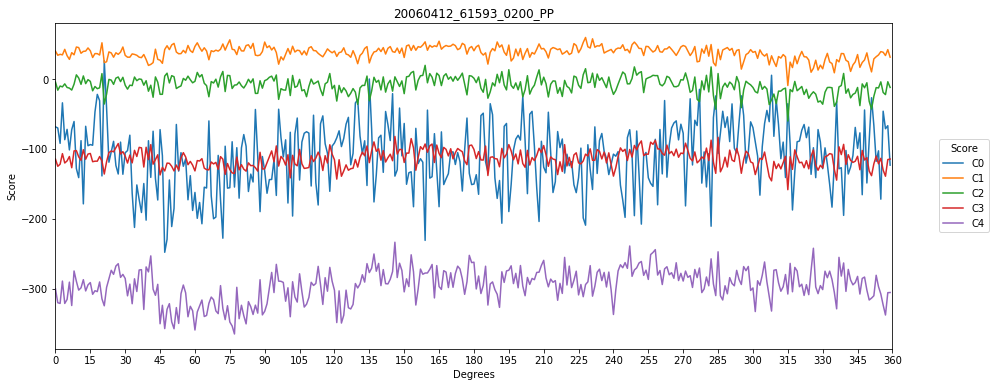
\includegraphics[width=\textwidth]{Figures/chapter_stability/20060412_61593_0200_PP/r/scores.png}
		\caption{Messidor 20060412 61593 0200 PP Tag: 1}
	\end{subfigure}
	\begin{subfigure}[b]{ 0.85\textwidth}
		\centering
		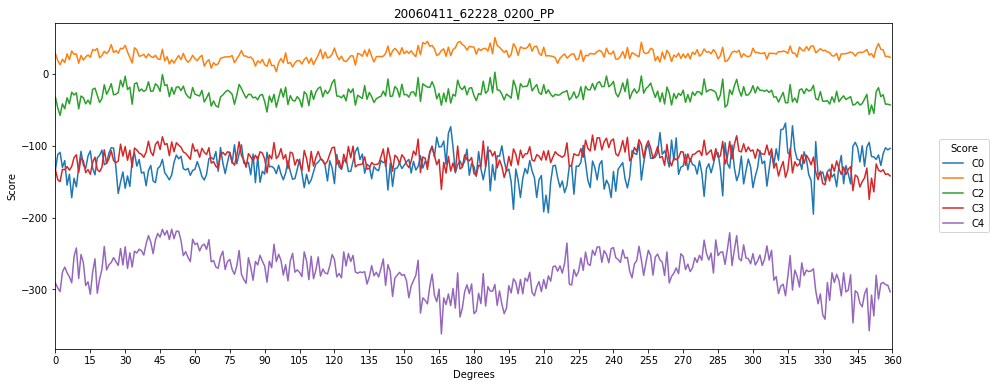
\includegraphics[width=\textwidth]{Figures/chapter_stability/20060411_62228_0200_PP/r/scores.png}
		\caption{Messidor 20060411 62228 0200 PP Tag: 1}		
	\end{subfigure}	
	\begin{subfigure}[b]{ 0.85\textwidth}
		\centering
		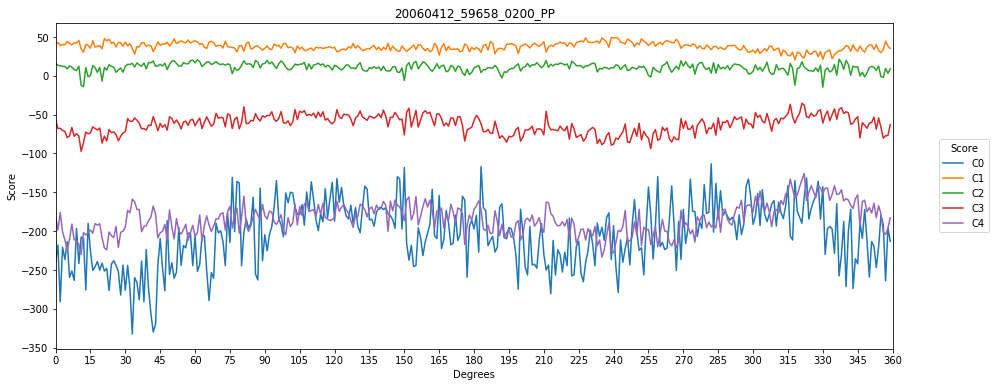
\includegraphics[width=\textwidth]{Figures/chapter_stability/20060412_59658_0200_PP/r/scores.png}
		\caption{Messidor 20060412 59658 0200 PP Tag: 1}		
	\end{subfigure}
	\begin{subfigure}[b]{ 0.85\textwidth}
		\centering
		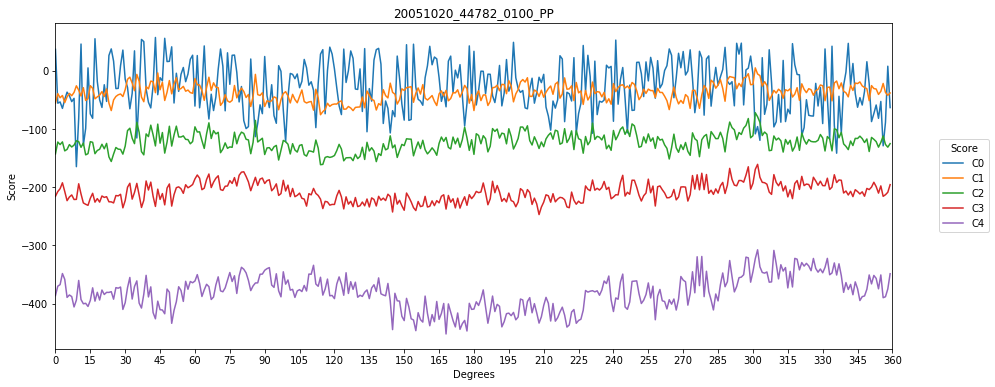
\includegraphics[width=\textwidth]{Figures/chapter_stability/20051020_44782_0100_PP/r/scores.png}
		\caption{Messidor 20051020 44782 0100 PP Tag: 1}		
	\end{subfigure}
	%}
	\hfill 
	\caption[Score vs Rotation (Tag: 1)]{Class Score vs Input Rotation (Tag: 1)}  
	\label{sta:fig:rot1} 
\end{figure}

\begin{figure}[ht!]
	\centering
	%\scalebox{0.9}{
	\begin{subfigure}[b]{ 0.85\textwidth}
		\centering
		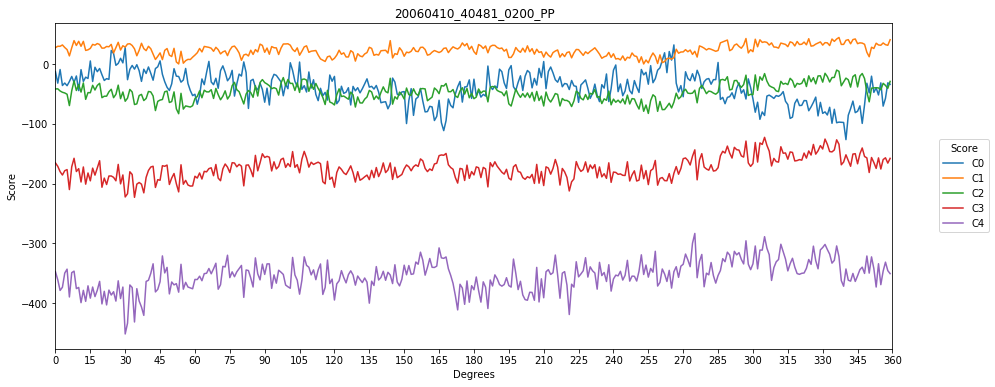
\includegraphics[width=\textwidth]{Figures/chapter_stability/20060410_40481_0200_PP/r/scores.png}
		\caption{Messidor 20060410 40481 0200 PP Tag: 2}		
	\end{subfigure}
	\begin{subfigure}[b]{ 0.85\textwidth}
		\centering
		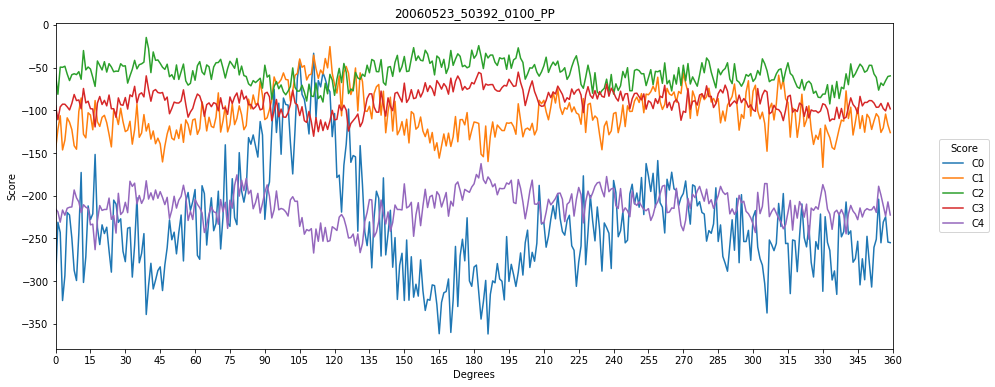
\includegraphics[width=\textwidth]{Figures/chapter_stability/20060523_50392_0100_PP/r/scores.png}
		\caption{Messidor 20060523 50392 0100 PP Tag: 2}		
	\end{subfigure}

	\begin{subfigure}[b]{ 0.85\textwidth}
		\centering
		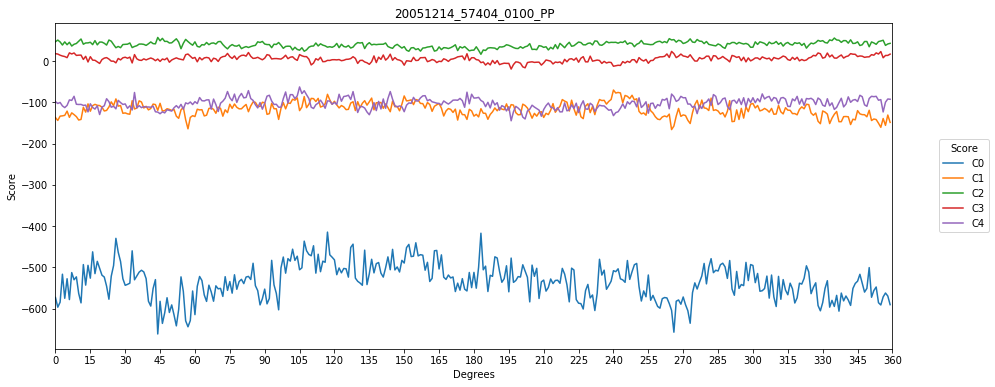
\includegraphics[width=\textwidth]{Figures/chapter_stability/20051214_57404_0100_PP/r/scores.png}
		\caption{Messidor 20051214 57404 0100 PP Tag: 2}		
	\end{subfigure}	
	\begin{subfigure}[b]{ 0.85\textwidth}
		\centering
		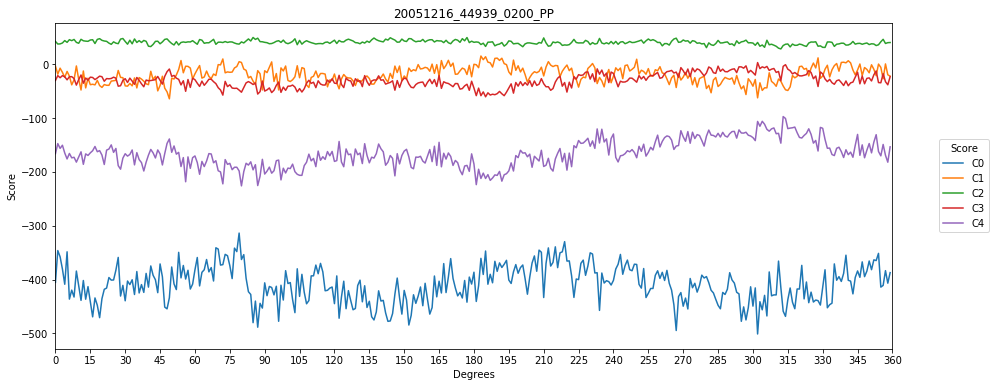
\includegraphics[width=\textwidth]{Figures/chapter_stability/20051216_44939_0200_PP/r/scores.png}
		\caption{Messidor 20051216 44939 0200 PP Tag: 2}		
	\end{subfigure}
	%}
	\hfill 
	\caption[Score vs Rotation (Tag: 2)]{Class Score vs Input Rotation (Tag: 2)}  
	\label{sta:fig:rot2} 
\end{figure}

\begin{figure}[ht!]
	\centering
	%\scalebox{0.9}{
	\begin{subfigure}[b]{ 0.85\textwidth}
		\centering
		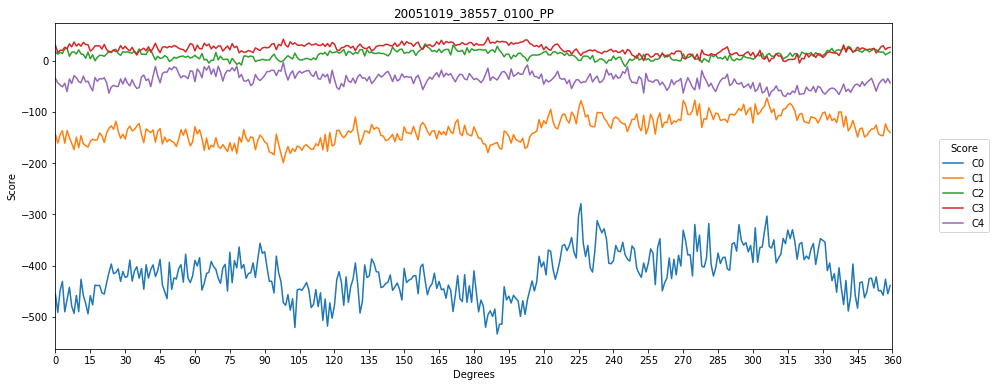
\includegraphics[width=\textwidth]{Figures/chapter_stability/20051019_38557_0100_PP/r/scores.png}
		\caption{Messidor 20051019 38557 0100 PP Tag: 3}				
	\end{subfigure}	
	\begin{subfigure}[b]{ 0.85\textwidth}
		\centering
		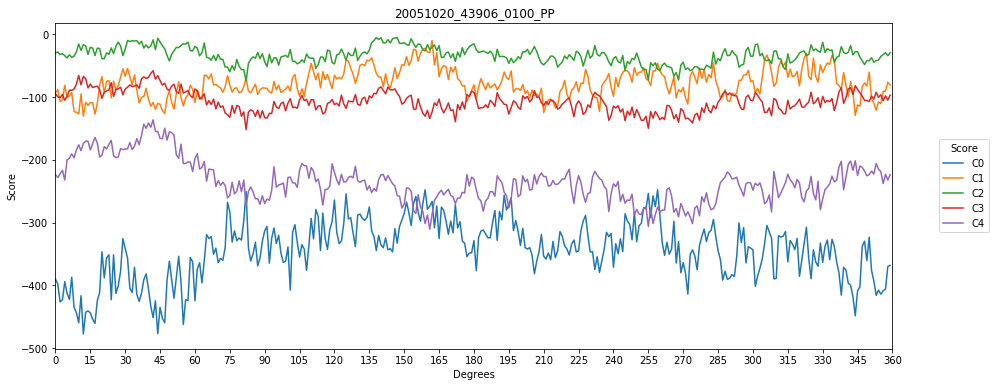
\includegraphics[width=\textwidth]{Figures/chapter_stability/20051020_43906_0100_PP/r/scores.png}
		\caption{Messidor 20051020 43906 0100 PP Tag: 3}				
	\end{subfigure}	
	\begin{subfigure}[b]{ 0.85\textwidth}
		\centering
		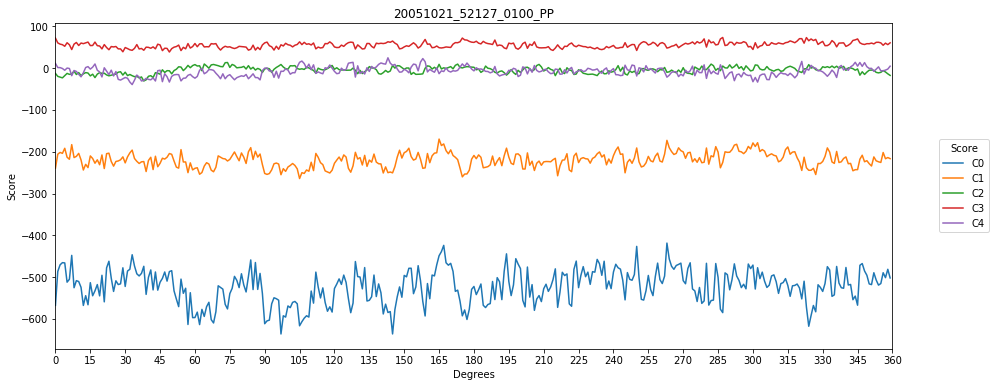
\includegraphics[width=\textwidth]{Figures/chapter_stability/20051021_52127_0100_PP/r/scores.png}
		\caption{Messidor 20051021 52127 0100 PP Tag: 3}				
	\end{subfigure}	
	\begin{subfigure}[b]{ 0.85\textwidth}
		\centering
		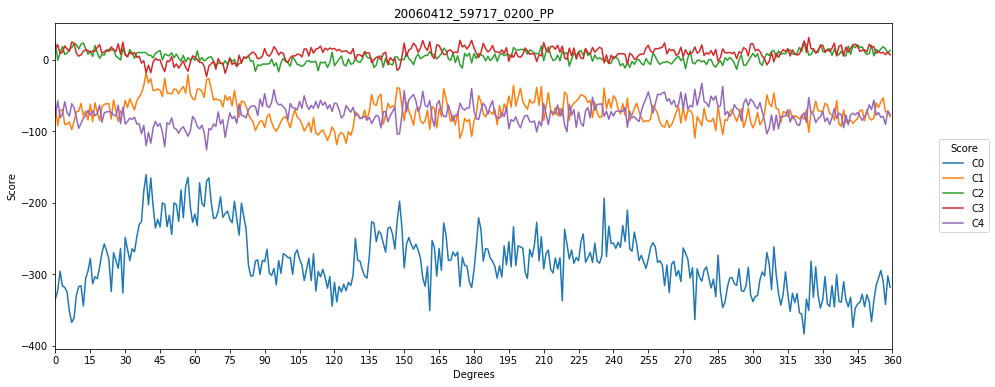
\includegraphics[width=\textwidth]{Figures/chapter_stability/20060412_59717_0200_PP/r/scores.png}
		\caption{Messidor 20060412 59717 0200 PP Tag: 3}		
	\end{subfigure}
	%}
	\hfill 
	\caption[Score vs Rotation (Tag: 3)]{Class Score vs Input Rotation (Tag: 3)}  
	\label{sta:fig:rot3} 
\end{figure}

\subsection{Lightness}

For all retina images a change in image lightness is applied maintaining constant hue and saturation. A broad change in lightness is studied going from 25\% of the original value of lightness to a 75\% more lightness. This variation helps to study the effect of light in the image in the predicted classes.

Figure \ref{sta:fig:lig0} shows the results for class 0 studied classes. For all four images a similar effect in score values of each class is observed for all the studied range of lightness following a parallel behavior under changes of lightness.

Figure \ref{sta:fig:lig1} shows the results for class 1 images. All score classes follow a similar change in the curves, being parallel between each other, except class 0 curve that consistently show higher values of its score relative to all other classes in both extremes of the lightness sprectrum. Either for dark or for too clear images, class 0 score increases respect all the other classes increasing the probability of false negatives in both extremes. The values of lightness under and above which class 0 score becomes the highest are 43 and 125 for first image, 30 and 125 forthe second, 38 for the third and 70 and 105 for the fourth. For all four images the predicted value under initial conditions is 1.

Figure \ref{sta:fig:lig2} shows the results for class 2 images. The effect of lightness is similar to the observed in previous cases, that is class 0 increasing in both extremes of the curve with one difference: the score signaling of class 2 and 3 are above the increase in value of class 0 scores. That's why only in the first case, that is predicted as class 1, a important reduction of lightness causes a false negative (under 40). In all other cases, the prediction is equal to the tag (class 2) showing a good stability under a high range of lightness.

Figure \ref{sta:fig:lig3} shows the results of class 3 images. Similar effects to the previous cases are observed that is, an increase of class 0 and 1 scores in the low and high lightness extremes, not being important under mild changes of lightness.

\begin{figure}[ht!]
	\centering
	%\scalebox{0.9}{
	\begin{subfigure}[b]{ 0.85\textwidth}
		\centering
		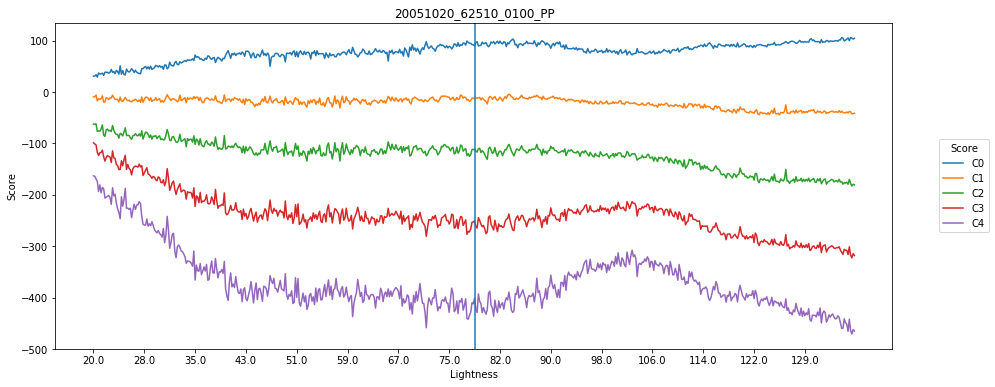
\includegraphics[width=\textwidth]{Figures/chapter_stability/20051020_62510_0100_PP/l/scores.png}
		\caption{Messidor 20051020 62510 0100 PP Tag: 0}
	\end{subfigure}
	\begin{subfigure}[b]{ 0.85\textwidth}
		\centering
		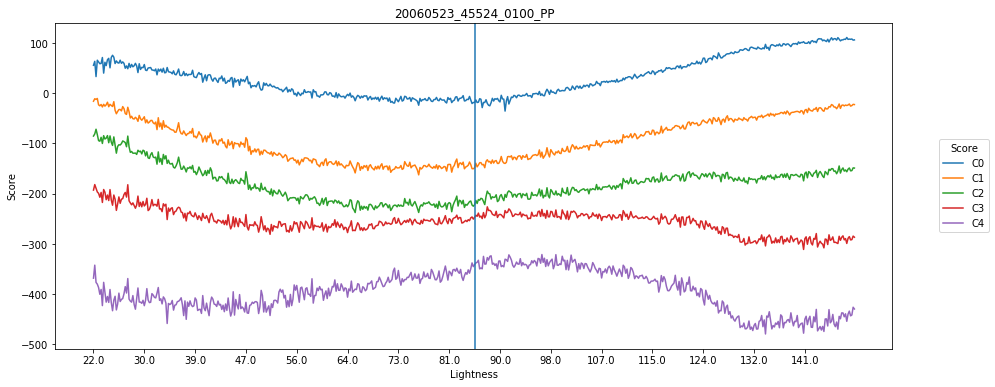
\includegraphics[width=\textwidth]{Figures/chapter_stability/20060523_45524_0100_PP/l/scores.png}
		\caption{Messidor 20060523 45524 0100 PP Tag: 0}		
	\end{subfigure}	
	\begin{subfigure}[b]{ 0.85\textwidth}
		\centering
		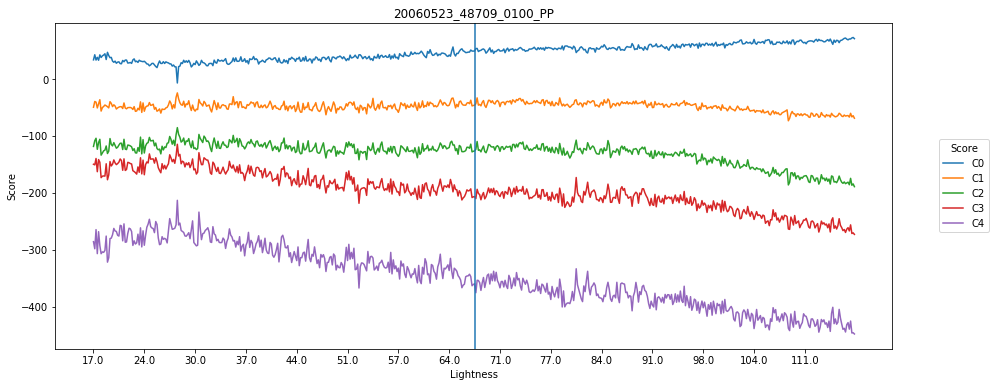
\includegraphics[width=\textwidth]{Figures/chapter_stability/20060523_48709_0100_PP/l/scores.png}
		\caption{Messidor 20060523 48709 0100 PP Tag: 0}		
	\end{subfigure}
	\begin{subfigure}[b]{ 0.85\textwidth}
		\centering
		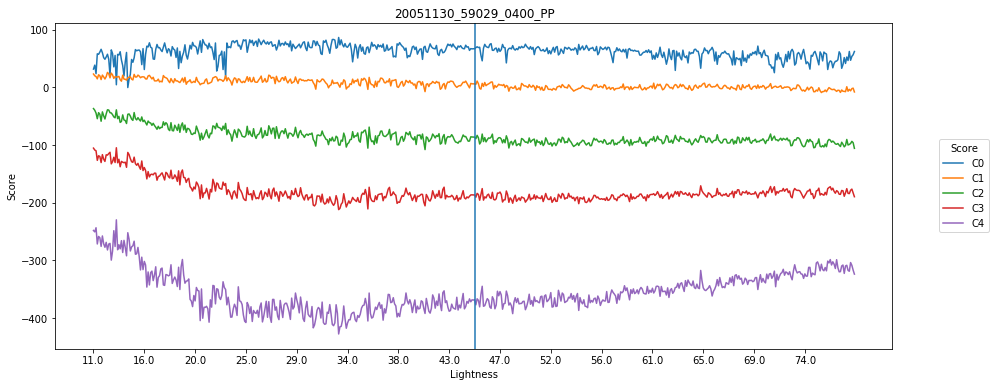
\includegraphics[width=\textwidth]{Figures/chapter_stability/20051130_59029_0400_PP/l/scores.png}
		\caption{Messidor 20051130 59029 0400 PP Tag: 0}		
	\end{subfigure}
	%}
	\hfill 
	\caption[Score vs Lightness (Tag: 0)]{Class Score vs Input Lightness (Tag: 0)}  
	\label{sta:fig:lig0} 
\end{figure}

\begin{figure}[ht!]
	\centering
	%\scalebox{0.9}{
	\begin{subfigure}[b]{ 0.85\textwidth}
		\centering
		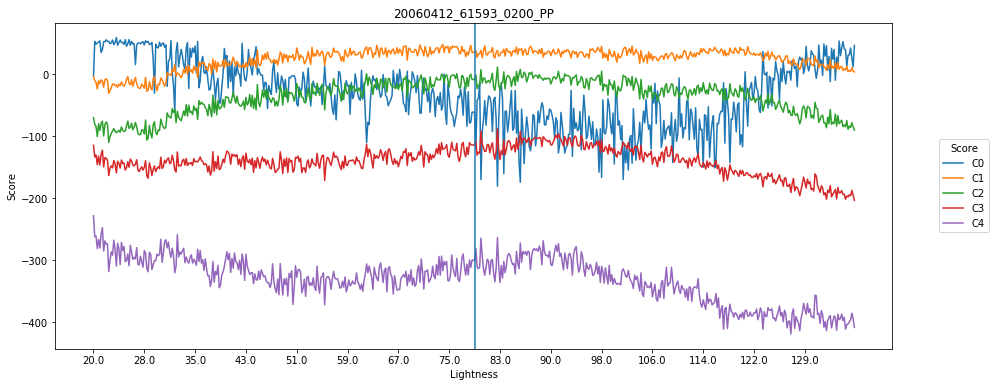
\includegraphics[width=\textwidth]{Figures/chapter_stability/20060412_61593_0200_PP/l/scores.png}
		\caption{Messidor 20060412 61593 0200 PP Tag: 1}
	\end{subfigure}
	\begin{subfigure}[b]{ 0.85\textwidth}
		\centering
		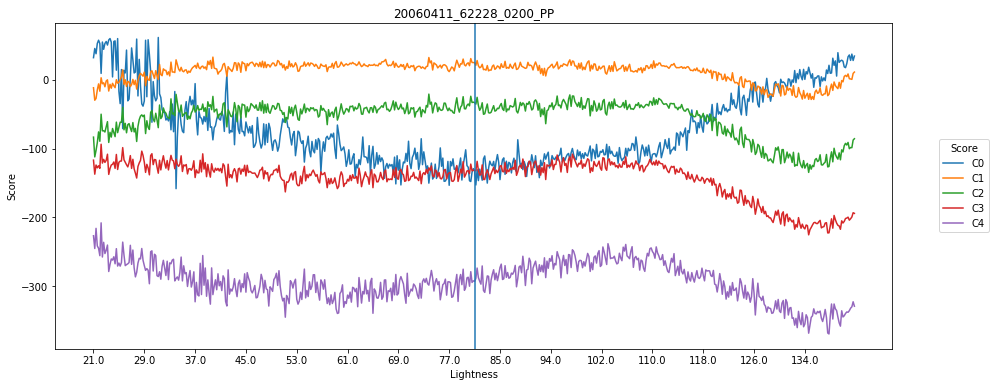
\includegraphics[width=\textwidth]{Figures/chapter_stability/20060411_62228_0200_PP/l/scores.png}
		\caption{Messidor 20060411 62228 0200 PP Tag: 1}		
	\end{subfigure}	
	\begin{subfigure}[b]{ 0.85\textwidth}
		\centering
		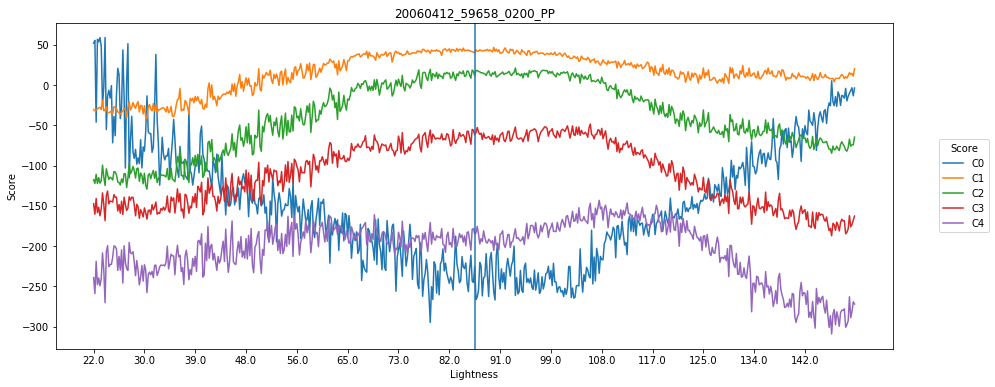
\includegraphics[width=\textwidth]{Figures/chapter_stability/20060412_59658_0200_PP/l/scores.png}
		\caption{Messidor 20060412 59658 0200 PP Tag: 1}		
	\end{subfigure}
	\begin{subfigure}[b]{ 0.85\textwidth}
		\centering
		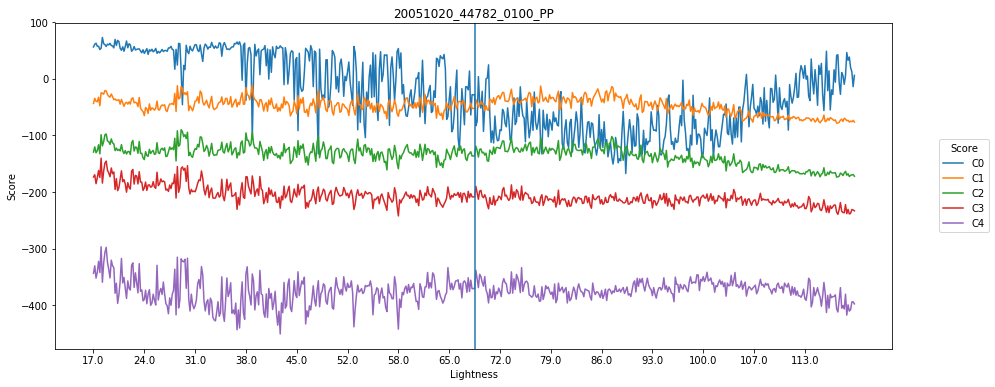
\includegraphics[width=\textwidth]{Figures/chapter_stability/20051020_44782_0100_PP/l/scores.png}
		\caption{Messidor 20051020 44782 0100 PP Tag: 1}		
	\end{subfigure}
	%}
	\hfill 
	\caption[Score vs Lightness (Tag: 1)]{Class Score vs Input Lightness (Tag: 1)}  
	\label{sta:fig:lig1} 
\end{figure}

\begin{figure}[ht!]
	\centering
	%\scalebox{0.9}{
	\begin{subfigure}[b]{ 0.85\textwidth}
		\centering
		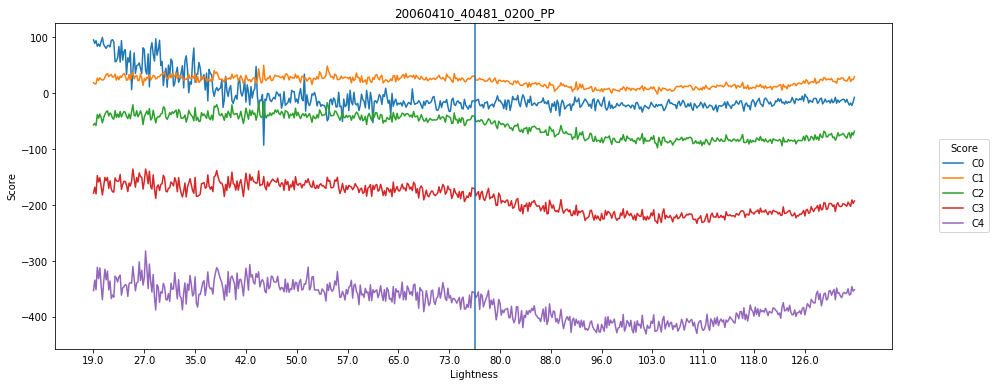
\includegraphics[width=\textwidth]{Figures/chapter_stability/20060410_40481_0200_PP/l/scores.png}
		\caption{Messidor 20060410 40481 0200 PP Tag: 2}		
	\end{subfigure}
	\begin{subfigure}[b]{ 0.85\textwidth}
		\centering
		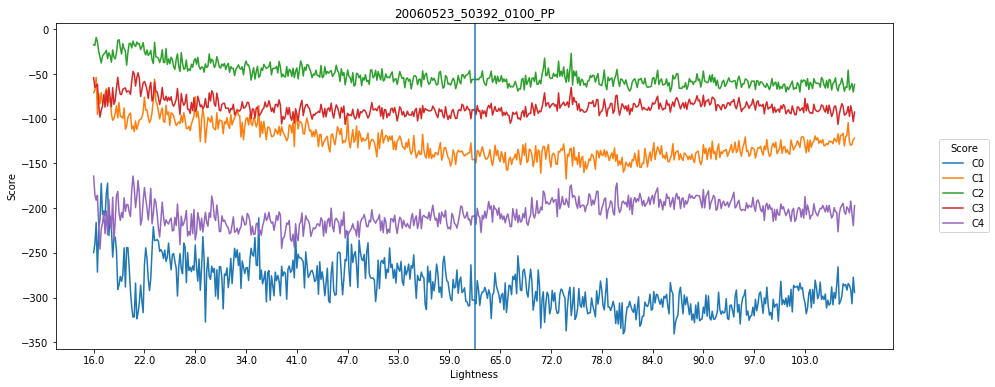
\includegraphics[width=\textwidth]{Figures/chapter_stability/20060523_50392_0100_PP/l/scores.png}
		\caption{Messidor 20060523 50392 0100 PP Tag: 2}		
	\end{subfigure}
	
	\begin{subfigure}[b]{ 0.85\textwidth}
		\centering
		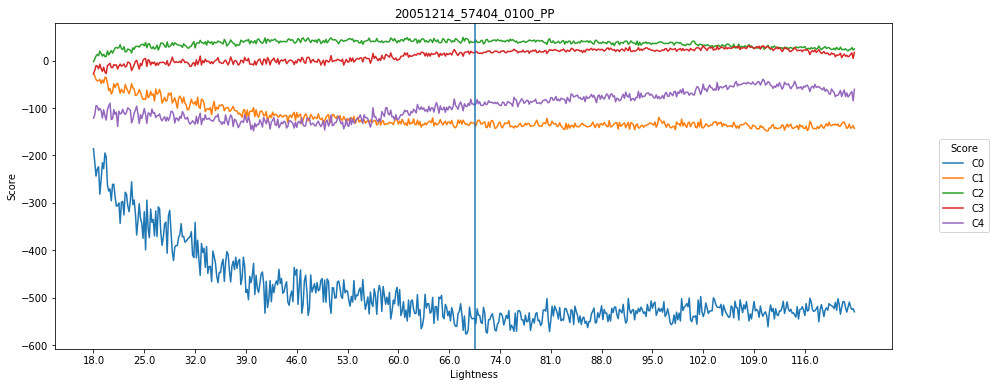
\includegraphics[width=\textwidth]{Figures/chapter_stability/20051214_57404_0100_PP/l/scores.png}
		\caption{Messidor 20051214 57404 0100 PP Tag: 2}		
	\end{subfigure}	
	\begin{subfigure}[b]{ 0.85\textwidth}
		\centering
		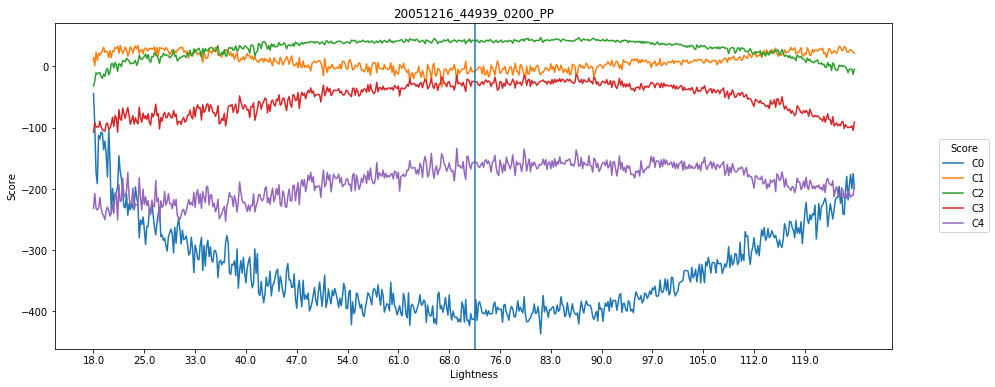
\includegraphics[width=\textwidth]{Figures/chapter_stability/20051216_44939_0200_PP/l/scores.png}
		\caption{Messidor 20051216 44939 0200 PP Tag: 2}		
	\end{subfigure}
	%}
	\hfill 
	\caption[Score vs Lightness (Tag: 2)]{Class Score vs Input Lightness (Tag: 2)}  
	\label{sta:fig:lig2} 
\end{figure}

\begin{figure}[ht!]
	\centering
	%\scalebox{0.9}{
	\begin{subfigure}[b]{ 0.85\textwidth}
		\centering
		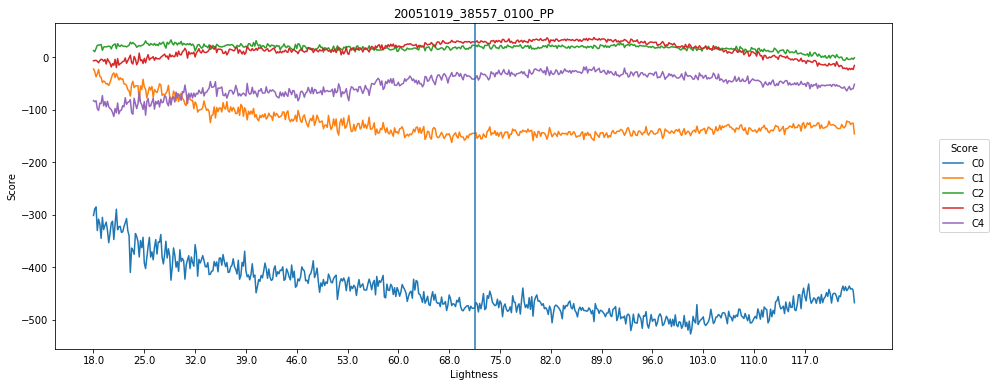
\includegraphics[width=\textwidth]{Figures/chapter_stability/20051019_38557_0100_PP/l/scores.png}
		\caption{Messidor 20051019 38557 0100 PP Tag: 3}				
	\end{subfigure}	
	\begin{subfigure}[b]{ 0.85\textwidth}
		\centering
		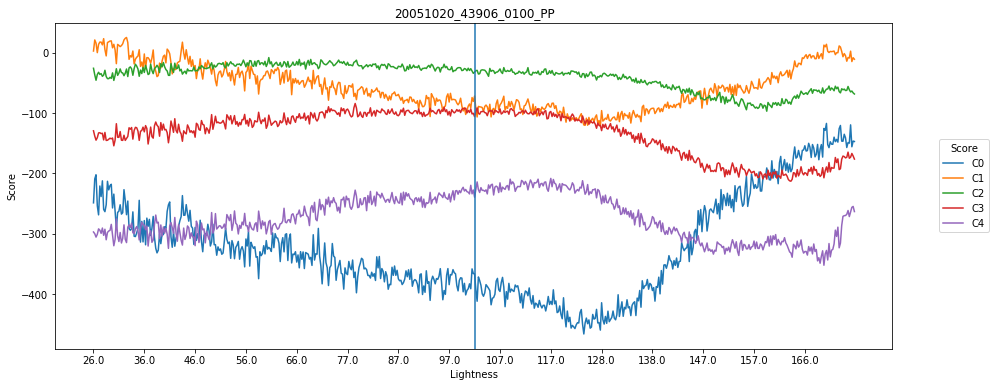
\includegraphics[width=\textwidth]{Figures/chapter_stability/20051020_43906_0100_PP/l/scores.png}
		\caption{Messidor 20051020 43906 0100 PP Tag: 3}				
	\end{subfigure}	
	\begin{subfigure}[b]{ 0.85\textwidth}
		\centering
		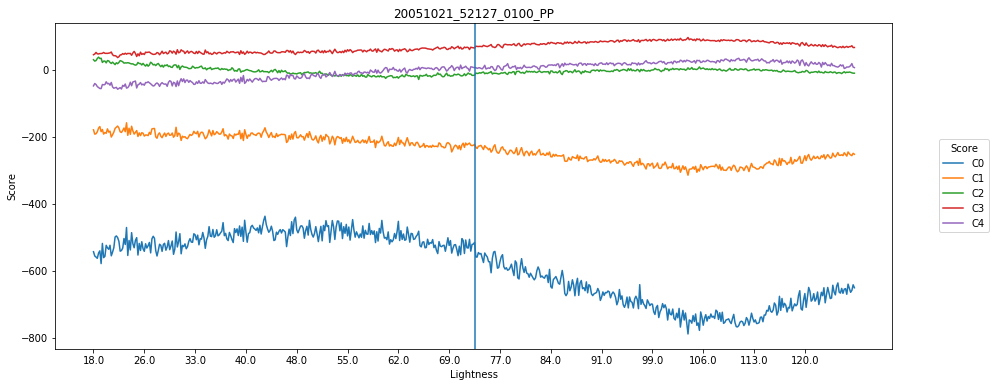
\includegraphics[width=\textwidth]{Figures/chapter_stability/20051021_52127_0100_PP/l/scores.png}
		\caption{Messidor 20051021 52127 0100 PP Tag: 3}				
	\end{subfigure}	
	\begin{subfigure}[b]{ 0.85\textwidth}
		\centering
		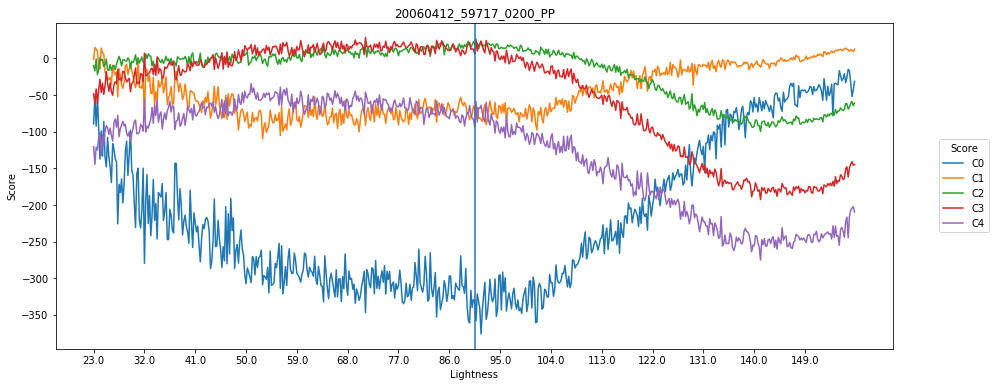
\includegraphics[width=\textwidth]{Figures/chapter_stability/20060412_59717_0200_PP/l/scores.png}
		\caption{Messidor 20060412 59717 0200 PP Tag: 3}		
	\end{subfigure}
	%}
	\hfill 
	\caption[Score vs Lightness (Tag: 3)]{Class Score vs Input Lightness (Tag: 3)}  
	\label{sta:fig:lig3} 
\end{figure}

\subsection{Saturation}

For all retina images a change in image saturation is applied maintaining constant hue and lightness. A broad change in saturation is studied going from 25\% less from original value to 75\% more saturation. This variation helps to study the effect of color saturation in the image in the predicted classes.

Figure \ref{sta:fig:sat0} shows the changes in predicted scores under different saturation degrees. No modification in predicted class is observed for the first three images. A change predicted class is observed in the last case for values of saturation under 90s.

Figures \ref{sta:fig:sat1}, \ref{sta:fig:sat2} and \ref{sta:fig:sat3},  show the scores for class 1, 2 and 3 images respectively. No significant changes are observed in the behavior of predicted classes, being the score maps flat in most of the cases.

\begin{figure}[ht!]
	\centering
	%\scalebox{0.9}{
	\begin{subfigure}[b]{ 0.85\textwidth}
		\centering
		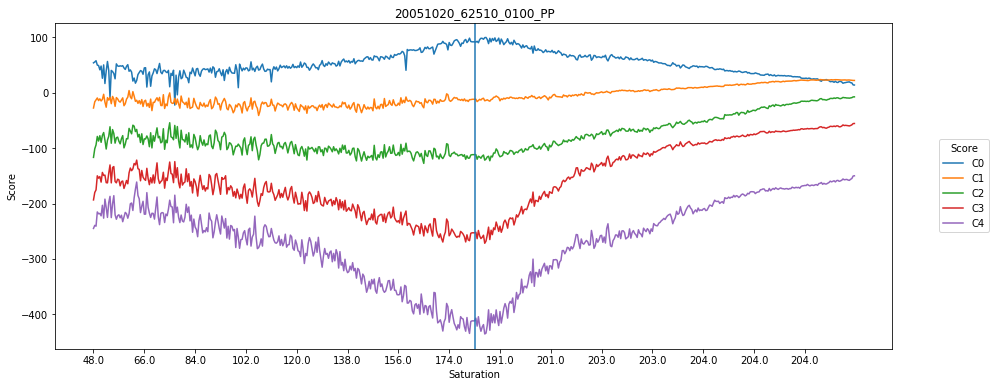
\includegraphics[width=\textwidth]{Figures/chapter_stability/20051020_62510_0100_PP/s/scores.png}
		\caption{Messidor 20051020 62510 0100 PP Tag: 0}
	\end{subfigure}
	\begin{subfigure}[b]{ 0.85\textwidth}
		\centering
		\includegraphics[width=\textwidth]{Figures/chapter_stability/20060523_45524_0100_PP/s/scores.png}
		\caption{Messidor 20060523 45524 0100 PP Tag: 0}		
	\end{subfigure}	
	\begin{subfigure}[b]{ 0.85\textwidth}
		\centering
		\includegraphics[width=\textwidth]{Figures/chapter_stability/20060523_48709_0100_PP/s/scores.png}
		\caption{Messidor 20060523 48709 0100 PP Tag: 0}		
	\end{subfigure}
	\begin{subfigure}[b]{ 0.85\textwidth}
		\centering
		\includegraphics[width=\textwidth]{Figures/chapter_stability/20051130_59029_0400_PP/s/scores.png}
		\caption{Messidor 20051130 59029 0400 PP Tag: 0}		
	\end{subfigure}
	%}
	\hfill 
	\caption[Score vs Saturation (Tag: 0)]{Class Score vs Input Saturation (Tag: 0)}  
	\label{sta:fig:sat0} 
\end{figure}

\begin{figure}[ht!]
	\centering
	%\scalebox{0.9}{
	\begin{subfigure}[b]{ 0.85\textwidth}
		\centering
		\includegraphics[width=\textwidth]{Figures/chapter_stability/20060412_61593_0200_PP/s/scores.png}
		\caption{Messidor 20060412 61593 0200 PP Tag: 1}
	\end{subfigure}
	\begin{subfigure}[b]{ 0.85\textwidth}
		\centering
		\includegraphics[width=\textwidth]{Figures/chapter_stability/20060411_62228_0200_PP/s/scores.png}
		\caption{Messidor 20060411 62228 0200 PP Tag: 1}		
	\end{subfigure}	
	\begin{subfigure}[b]{ 0.85\textwidth}
		\centering
		\includegraphics[width=\textwidth]{Figures/chapter_stability/20060412_59658_0200_PP/s/scores.png}
		\caption{Messidor 20060412 59658 0200 PP Tag: 1}		
	\end{subfigure}
	\begin{subfigure}[b]{ 0.85\textwidth}
		\centering
		\includegraphics[width=\textwidth]{Figures/chapter_stability/20051020_44782_0100_PP/s/scores.png}
		\caption{Messidor 20051020 44782 0100 PP Tag: 1}		
	\end{subfigure}
	%}
	\hfill 
	\caption[Score vs Saturation (Tag: 1)]{Class Score vs Input Saturation (Tag: 1)}  
	\label{sta:fig:sat1} 
\end{figure}

\begin{figure}[ht!]
	\centering
	%\scalebox{0.9}{
	\begin{subfigure}[b]{ 0.85\textwidth}
		\centering
		\includegraphics[width=\textwidth]{Figures/chapter_stability/20060410_40481_0200_PP/s/scores.png}
		\caption{Messidor 20060410 40481 0200 PP Tag: 2}		
	\end{subfigure}
	\begin{subfigure}[b]{ 0.85\textwidth}
		\centering
		\includegraphics[width=\textwidth]{Figures/chapter_stability/20060523_50392_0100_PP/s/scores.png}
		\caption{Messidor 20060523 50392 0100 PP Tag: 2}		
	\end{subfigure}
	
	\begin{subfigure}[b]{ 0.85\textwidth}
		\centering
		\includegraphics[width=\textwidth]{Figures/chapter_stability/20051214_57404_0100_PP/s/scores.png}
		\caption{Messidor 20051214 57404 0100 PP Tag: 2}		
	\end{subfigure}	
	\begin{subfigure}[b]{ 0.85\textwidth}
		\centering
		\includegraphics[width=\textwidth]{Figures/chapter_stability/20051216_44939_0200_PP/s/scores.png}
		\caption{Messidor 20051216 44939 0200 PP Tag: 2}		
	\end{subfigure}
	%}
	\hfill 
	\caption[Score vs Saturation (Tag: 2)]{Class Score vs Input Saturation (Tag: 2)}  
	\label{sta:fig:sat2} 
\end{figure}

\begin{figure}[ht!]
	\centering
	%\scalebox{0.9}{
	\begin{subfigure}[b]{ 0.85\textwidth}
		\centering
		\includegraphics[width=\textwidth]{Figures/chapter_stability/20051019_38557_0100_PP/s/scores.png}
		\caption{Messidor 20051019 38557 0100 PP Tag: 3}				
	\end{subfigure}	
	\begin{subfigure}[b]{ 0.85\textwidth}
		\centering
		\includegraphics[width=\textwidth]{Figures/chapter_stability/20051020_43906_0100_PP/s/scores.png}
		\caption{Messidor 20051020 43906 0100 PP Tag: 3}				
	\end{subfigure}	
	\begin{subfigure}[b]{ 0.85\textwidth}
		\centering
		\includegraphics[width=\textwidth]{Figures/chapter_stability/20051021_52127_0100_PP/s/scores.png}
		\caption{Messidor 20051021 52127 0100 PP Tag: 3}				
	\end{subfigure}	
	\begin{subfigure}[b]{ 0.85\textwidth}
		\centering
		\includegraphics[width=\textwidth]{Figures/chapter_stability/20060412_59717_0200_PP/s/scores.png}
		\caption{Messidor 20060412 59717 0200 PP Tag: 3}		
	\end{subfigure}
	%}
	\hfill 
	\caption[Score vs Saturation (Tag: 3)]{Class Score vs Input Saturation (Tag: 3)}  
	\label{sta:fig:sat3} 
\end{figure}

\subsection{Hue}

Hue is the studied variable having the most important influence on class prediction. This is an expected result due to its nature. Hue angle represents color, being such property the most important characteristic used for differentiating lesions, thus the model is expected to use color information for score determination. Extreme hue values far from true values give the higher score to class 0. Only in a narrow range between the original values the model is able to find the correct classification. Figures \ref{sta:fig:hue0}, \ref{sta:fig:hue1}, \ref{sta:fig:hue2} and \ref{sta:fig:hue3} show the score representations for changes in hue. The pattern observed is the same for all images of all classes.

\begin{figure}[ht!]
	\centering
	%\scalebox{0.9}{
	\begin{subfigure}[b]{ 0.85\textwidth}
		\centering
		\includegraphics[width=\textwidth]{Figures/chapter_stability/20051020_62510_0100_PP/h/scores.png}
		\caption{Messidor 20051020 62510 0100 PP Tag: 0}
	\end{subfigure}
	\begin{subfigure}[b]{ 0.85\textwidth}
		\centering
		\includegraphics[width=\textwidth]{Figures/chapter_stability/20060523_45524_0100_PP/h/scores.png}
		\caption{Messidor 20060523 45524 0100 PP Tag: 0}		
	\end{subfigure}	
	\begin{subfigure}[b]{ 0.85\textwidth}
		\centering
		\includegraphics[width=\textwidth]{Figures/chapter_stability/20060523_48709_0100_PP/h/scores.png}
		\caption{Messidor 20060523 48709 0100 PP Tag: 0}		
	\end{subfigure}
	\begin{subfigure}[b]{ 0.85\textwidth}
		\centering
		\includegraphics[width=\textwidth]{Figures/chapter_stability/20051130_59029_0400_PP/h/scores.png}
		\caption{Messidor 20051130 59029 0400 PP Tag: 0}		
	\end{subfigure}
	%}
	\hfill 
	\caption[Score vs Hue (Tag: 0)]{Class Score vs Input Hue (Tag: 0)}  
	\label{sta:fig:hue0} 
\end{figure}

\begin{figure}[ht!]
	\centering
	%\scalebox{0.9}{
	\begin{subfigure}[b]{ 0.85\textwidth}
		\centering
		\includegraphics[width=\textwidth]{Figures/chapter_stability/20060412_61593_0200_PP/h/scores.png}
		\caption{Messidor 20060412 61593 0200 PP Tag: 1}
	\end{subfigure}
	\begin{subfigure}[b]{ 0.85\textwidth}
		\centering
		\includegraphics[width=\textwidth]{Figures/chapter_stability/20060411_62228_0200_PP/h/scores.png}
		\caption{Messidor 20060411 62228 0200 PP Tag: 1}		
	\end{subfigure}	
	\begin{subfigure}[b]{ 0.85\textwidth}
		\centering
		\includegraphics[width=\textwidth]{Figures/chapter_stability/20060412_59658_0200_PP/h/scores.png}
		\caption{Messidor 20060412 59658 0200 PP Tag: 1}		
	\end{subfigure}
	\begin{subfigure}[b]{ 0.85\textwidth}
		\centering
		\includegraphics[width=\textwidth]{Figures/chapter_stability/20051020_44782_0100_PP/h/scores.png}
		\caption{Messidor 20051020 44782 0100 PP Tag: 1}		
	\end{subfigure}
	%}
	\hfill 
	\caption[Score vs Hue (Tag: 1)]{Class Score vs Input Hue (Tag: 1)}  
	\label{sta:fig:hue1} 
\end{figure}

\begin{figure}[ht!]
	\centering
	%\scalebox{0.9}{
	\begin{subfigure}[b]{ 0.85\textwidth}
		\centering
		\includegraphics[width=\textwidth]{Figures/chapter_stability/20060410_40481_0200_PP/h/scores.png}
		\caption{Messidor 20060410 40481 0200 PP Tag: 2}		
	\end{subfigure}
	\begin{subfigure}[b]{ 0.85\textwidth}
		\centering
		\includegraphics[width=\textwidth]{Figures/chapter_stability/20060523_50392_0100_PP/h/scores.png}
		\caption{Messidor 20060523 50392 0100 PP Tag: 2}		
	\end{subfigure}
	
	\begin{subfigure}[b]{ 0.85\textwidth}
		\centering
		\includegraphics[width=\textwidth]{Figures/chapter_stability/20051214_57404_0100_PP/h/scores.png}
		\caption{Messidor 20051214 57404 0100 PP Tag: 2}		
	\end{subfigure}	
	\begin{subfigure}[b]{ 0.85\textwidth}
		\centering
		\includegraphics[width=\textwidth]{Figures/chapter_stability/20051216_44939_0200_PP/h/scores.png}
		\caption{Messidor 20051216 44939 0200 PP Tag: 2}		
	\end{subfigure}
	%}
	\hfill 
	\caption[Score vs Hue (Tag: 2)]{Class Score vs Input Hue (Tag: 2)}  
	\label{sta:fig:hue2} 
\end{figure}

\begin{figure}[ht!]
	\centering
	%\scalebox{0.9}{
	\begin{subfigure}[b]{ 0.85\textwidth}
		\centering
		\includegraphics[width=\textwidth]{Figures/chapter_stability/20051019_38557_0100_PP/h/scores.png}
		\caption{Messidor 20051019 38557 0100 PP Tag: 3}				
	\end{subfigure}	
	\begin{subfigure}[b]{ 0.85\textwidth}
		\centering
		\includegraphics[width=\textwidth]{Figures/chapter_stability/20051020_43906_0100_PP/h/scores.png}
		\caption{Messidor 20051020 43906 0100 PP Tag: 3}				
	\end{subfigure}	
	\begin{subfigure}[b]{ 0.85\textwidth}
		\centering
		\includegraphics[width=\textwidth]{Figures/chapter_stability/20051021_52127_0100_PP/h/scores.png}
		\caption{Messidor 20051021 52127 0100 PP Tag: 3}				
	\end{subfigure}	
	\begin{subfigure}[b]{ 0.85\textwidth}
		\centering
		\includegraphics[width=\textwidth]{Figures/chapter_stability/20060412_59717_0200_PP/h/scores.png}
		\caption{Messidor 20060412 59717 0200 PP Tag: 3}		
	\end{subfigure}
	%}
	\hfill 
	\caption[Score vs Hue (Tag: 3)]{Class Score vs Input Hue (Tag: 3)}  
	\label{sta:fig:hue3} 
\end{figure}
%----------------------------------------------------------------------------------------
%	SECTION 2
%----------------------------------------------------------------------------------------

\section{Conclusions}

The objective of this chapter was to study the capabilities and limitations of the classification model designed in chapter \ref{Chapter:Ordinal_Regression}. For this purpose a test of the robustness of its results has been done applying different changes to the inputs, in order to determine the important elements that have to be taken into account in inference time. The chosen properties of study have been: rotation, lightness, saturation and hue. A set of four random images of each class have been selected and modified according to the properties of study. A graphical representation of each variable versus scores have been generated in order to study the influence of each one of such variables in predicted classes.

From this analysis we have made several observations:

\begin{enumerate}[label=\Alph*)]

\item The model shows a high robustness to changes in rotation. One evaluation is enough in most of the cases, allowing only a slight improvement in statistical results when more than one evaluation is used. This means that is not necessary to rotate the image in order to improve the classification results. It also means that if the photo is taken in different rotations, the classifier works also correctly.

\item Lightness extremes cause an increase in class 0 scores that could produce false negatives. Such effect is less important when predicting images of classes greater than 1, because the signals produced by the positive detection is higher than the increase in class 0 scores, produced by lightness extreme values. These results show that model is highly robust to changes in image illumination. This study also produced a range on lightness variation that could be used to decide if an image has the proper illumination condition to be used for inferring a classification or if must be discarded.

\item Saturation does not seem to have an important effect on predicted scores. Most of the generated maps are flat. We can conclude then that model is robust to changes in input image saturation.

\item Hue is critical for the model. The model only work well under certain intervals. This result is consistent with experts use of color information to differentiate between aneurysms, exhudates, and other disease related lesions. The color of such lesions is also related to vessels color and the eye fundus color (as well as macula). Therefore, altering hue has a great impact on the features used by the model for lesion identification. However, hue variations are a change difficult to have with well calibrated cameras.

\end{enumerate}

This type of studies allows the identification of strengths and weaknesses of the models. Other variables could also be studied, like for example zoom, original image resolution, etc. to have a prior knowledge about model behavior under certain input conditions that may occur in inference time. However, we have not considered such studies because, due to the nature of our problem, we can assure to have a fixed resolution and zoom in our input images.

